% the first part of the document before the begin is called preamble
\documentclass[12pt, a4paper]{article}
\usepackage{graphicx}
\graphicspath{ {./images/} }
%
\author{Leonardo Valente}
\title{Sistemi Distribuiti}

\begin{document}
    \maketitle
    \tableofcontents
    \section{Introduzione}
    \subsection{Che cosa è un sistema distribuito?}
    
    Ci possono essere diverse definizioni di ''Sistema Distributo''.
    \begin{itemize}
        \item Definiamo un sistema distribuito come un insieme di componenti 
        Hardware e Software localizzati in una rete di computer che
        comunicano e coordinano le loro azioni solo passandosi messaggi.
        
        \item Un ''Sistema Distribuito'' è un insieme di elementi di computazione
        autonomi che appaiono all'utente come un singolo sistema coerente.
    \end{itemize}

    \subsection{Caratteristiche}
    Gli "elementi di computazione autonoma" di un SD, anche chiamati "Nodi"
    sono i device hardware oppure i processi software. Il fatto un SD debba sembrare
    un singolo sistema all'utente implica il fatto che tra i nodi ci deve essere un sistema
    di collaborazione.
    \\
    Quindi ogni nodo in quanto autonomo avrà la sua singola nozione di tempo. 
    Non esiste un clock globable per tutti i nodi.
    \\
    Questo porta quindi a problemi di sincronizzazione e di coordinamento.
    \\\\
    La parola chiave resta sempre: \textbf{Trasparenza}
    \\\\E' inevitabile il fatto che in qualsiasi momento solo parte del sistema fallirà.
    Nascondere questi fallimenti e il loro recupero è molto spesso difficile e in generale impossibile da nascondere.
    \\\\
    \textbf{Gestione della memoria?}
    
    \begin{itemize}
        \item Non c'è memoria condivisa.
        \item Comunicazione via scambio di messaggi.
        \item Ogni componente conosce solo il proprio stato e può sondare lo stato degli altri
    \end{itemize}
    \textbf{Gestione dell' esecuzione?}
    \begin{itemize}
        \item Ogni componente è autonomo.
        \item Il coordinamento delle attività è importante per il funzionamento di un sistema
        formato da più componenti.
    \end{itemize}
    \textbf{Gestione dell tempo?}
    \begin{itemize}
        \item Non c'è un clock globale.
        \item Non c'è possibilità di scheduling globale.
    \end{itemize}
    \textbf{Tipi di fallimenti}
    \begin{itemize}
        \item Fallimenti indipendenti dei singoli nodi.
        \item Non c'è fallimento globale.
    \end{itemize}
    
    \subsection{Gruppi}
    I gruppi possono essere \textbf{aperti} (tutti i nodi possono partecipare)
    o \textbf{chiusi} (solo membri selezionati possono partecipare).
  
     
    \section{Architetture Software}
    Una architettura software definisce la struttura del sistema,
    le interfacce tra i componenti e i pattern di interazione.
    \\
    Ci possono essere diversi stili di architettura per un SD.
    \begin{itemize}
        \item \textbf{Architetture a strati} (layered)\\Ho un livello superiore che nasconde
        il lavoro effettuato dal livello sottostante.
    \end{itemize}
    \begin{itemize}
        \item \textbf{Architetture a livelli}\\Applicazioni client server.
    \end{itemize}
    \begin{itemize}
        \item \textbf{Architetture basate sugli oggetti}
    \end{itemize}
    \begin{itemize}
        \item \textbf{Architetture basate su eventi}\\Applicazioni web dinamiche basate su callback (AJAX).
    \end{itemize}
    
    \subsection{Tipi di layer}

    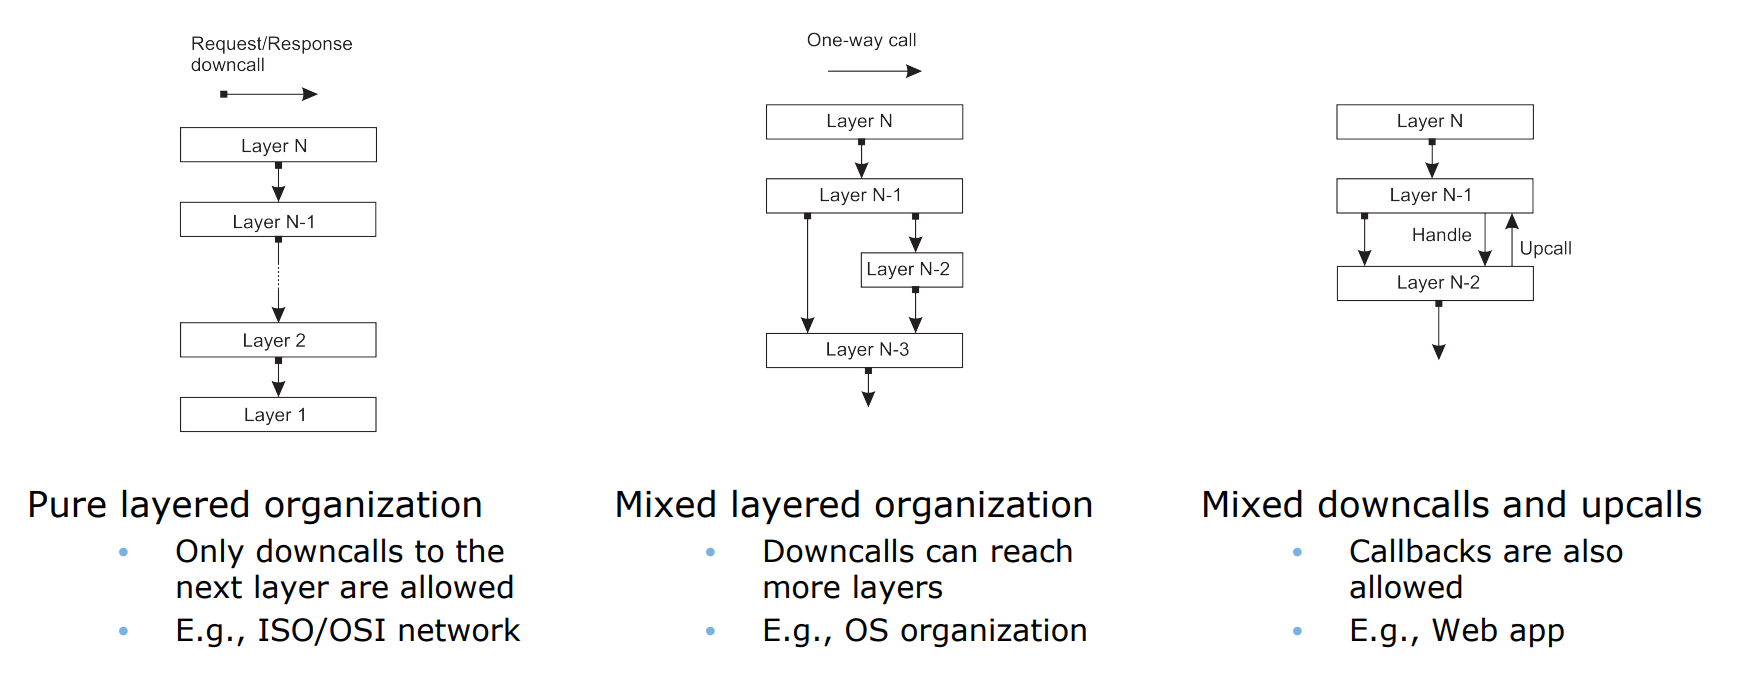
\includegraphics[scale=0.32]{layered.png}

    \begin{itemize}
        \item Il primo caso è molto semplice. Abbiamo a disposizione N livelli di layer, ognuno che comunica
        solo ed esclusivamente con il livello sottostante.
        \item Il secondo caso invece potrebbe risultare un po più complicato. Per spiegarlo usiamo un semplice esempio:
        supponiamo che il nostro programma effettui una operazione di divisione per 0 (zero).
        Ovviamente sappiamo che ciò non è possibile, quindi passerà il compito di risolvere questa eccezione
        all'exception handler e successivamente tornerà a fare quello che doveva fare.
        Invece se effettuiamo una normale operazione che non genera eccezzioni ovviamente non dovrà fare la parte dell'exception handler.
        \item Per il terzo caso basti immaginare a come funziona AJAX o più in generale il funzionamento di una web app.
        Quindi chiamate al server con eventuale risposta e aggiornamento della UI.
    \end{itemize}

    \subsection{Diversi tipi di Sistemi Distribuiti}
    E' importante differenziare i 3 tipi principali di SD.
    \begin{itemize}
        \item DOS (Distributed Operating System)
        \item NOS (Network Operating System)
        \item Middleware
    \end{itemize}  
    
    \subsection*{Distributed Operating System}
    L'utente non è a conoscenza della molteplicità delle macchine che compongono il sistema.
    \\I dati possono essere spostanti in modo intero o parziale, così come le operazioni di computazione.
    \\Un processo può essere migrato interamente o in modo parziale su diversi siti, facendo così avremo un effetto
    di \textbf{Load balancing}, che ci permette di distribuire il carico di lavoro su più macchine, 
    e di \textbf{Compuatation speedup} (i sottoprocessi possono essere eseguiti concorrentemente su più siti).
    Però il processo potrebbe aver bisogno di un determinato hardware (\textbf{Hardware preference}) oppure
    di un determinato software (\textbf{Software preference}). Avendo la possibilità di migrare il processo
    questo può essere possibile. 
    Infine il processo può essere eseguito in modo remoto, invece che trasferire i dati in locale.
    \newpage
    \subsection*{Network Operating System}
    L'utente è a conoscenza della molteplicità delle macchine che compongono il sistema.
    \\NOS permette operazioni esplicite di comunicazione: \textbf{Socket}.
    (Comunicazione diretta tra processi.)
    \\L'accesso alle risorse sulle varie macchine è effettuata in modo esplicito tramite:
    \begin{itemize}
        \item Remote logging (telnet, ssh)
        \item Remote desktop
        \item FTP
    \end{itemize}
    \subsection*{Middleware}
    Il compito del middleware è quello di implementare i servizi per renderli trasparenti all'applicazione.
    \begin{itemize}
        \item Definisce e offre un modello di comunicazione che nasconde i dettagli dei messaggi passati.
        \item Definisce e offre un servizio automatico per il salvataggio dei dati (su file system o DB).
        \item Definisce e offre un modello persistente per garantire consistenza su operazioni di lettura e scrittura (di solito su DB).
        \item Definisce e offre modelli di protezione nell'accesso ai dati e servizi.
    \end{itemize}
    \newpage
    \section{Il Modello Client-Server}

    \begin{figure}[htbp]
        \centering
        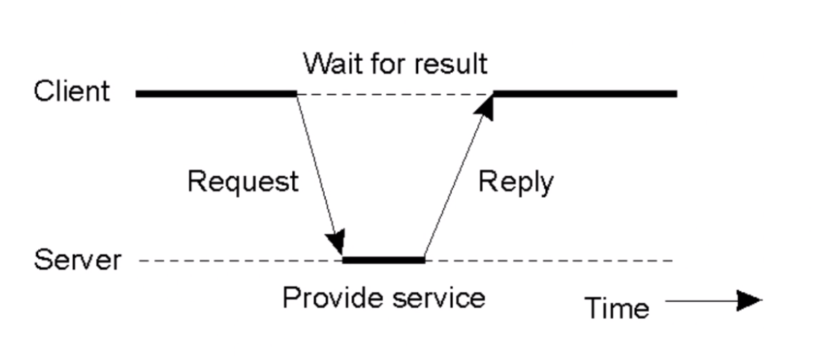
\includegraphics[scale=0.5]{clientserver.png}  
    \end{figure}
    Di base questa architettura prevede che un \textbf{client} acceda ad un \textbf{server} con
    una richiesta e che il server risponda con un risultato.
    \\Come possiamo notare dall'immagine, chiaramenta la richiesta con annessa risposta
    non è immediata, dovrà trascorrere un determinato quanto di tempo affinchè il server
    riesca a soddisfare la richiesta del client.
    \\\\
    Ci possono essere diversi tipi di modelli.

    \begin{itemize}
        \item \textbf{Accesso a Server multipli}.
        \\Il client accede ad un server che a sua volta può accedere ad un altro
        server. 
        \begin{figure}[htbp]
            \centering
            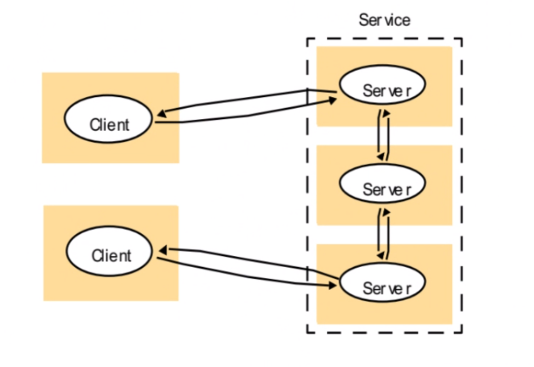
\includegraphics[scale=0.5]{servermultipli.png}  
        \end{figure}
        \newpage
        \item \textbf{Accesso via Proxy}
        \\Il \textit{Proxy} è un tipo di server che funge da intermediario per le richieste
        da parte di client alla ricerca di risorse su altri server.
        \\Il Server Proxy è molto utile per fornire l'anonimato durante la navigazione.
        \begin{figure}[htbp]
            \centering
            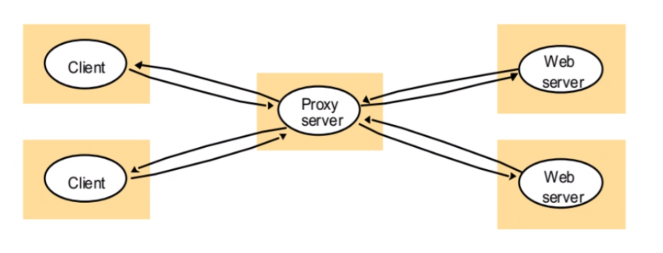
\includegraphics[scale=0.5]{proxy.png}  
        \end{figure}
    \end{itemize}
    
    \subsection{Problemi Fondamentali}
    In generale, ogni Sistema Distribuito deve aver a che fare con 4 problemi fondamentali:
    \begin{itemize}
        \item \textbf{Namig} (Identificare la controparte)
        \\Chi è la mia controparte? Dobbiamo assegnare dei nomi

        \item \textbf{Access point} (Accedere alla controparte)
        \\Come posso accedere ad una risorsa remota o un processo?

        \item \textbf{Protocol} (Comunicazione)
        \\Come posso scambiare messaggi? Bisogna mettersi d'accordo sul formato

        \item \textbf{Still an open issue} (Comunicazione)
        \\Come posso capire il contenuto di un messaggio?
    \end{itemize}

    \subsection{Trasparenza}
    Il concetto fondamentale alla base di un buon Sistema Distribuito è, appunto,
    la trasparenza. Per cui, per esempio, il come un particolare dato venga rappresentato
    e la metodologia di accesso a quel dato sono \textit{trasparenti} all'utente, non li vede.
    Così come anche la \textit{location}. Non sappiamo dove quel dato risiede fisicamente.
    \\\\Però, avere un \textbf{grado} di trasparenza troppo elevato potrebbe risultare eccessivo.
    Per esempio:
    \begin{itemize}
        \item Alcune \textit{latenze di comunicazione} non possono essere nascoste.
        \item Nascondere i fallimenti del sistema e dei nodi è talvolta \textbf{impossibile}.
        \item Esporre le distribuzioni potrebbe essere alcune volte una buona pratica.
        \\Se un server non dovesse rispondere ad una chiamata per troppo tempo, bisogna riportare il fallimento
        per dare un feedback all'utente di cosa sta accadendo e di agire di conseguenza.
        \item Inoltre, la trasparenza completa ha un costo elevato 
        (e.g.\ Mantenere le repliche di tutti i dati esattamente "up-to-date" con il master)
    \end{itemize}

    \subsubsection{Information Hiding}
    L'Information Hiding è il principio che sta alla base dell'\textit{Ingegneria del Software}.
    \\E' importante fare una distinzione tra:
    \begin{itemize}
        \item \textbf{cosa} un servizio o un sistema mette a disposizione
        \\definisce l'\textit{Application Programming Interface} (API) dei componenti o del sistema.
        \item \textbf{come} un servizio è stato implementato e distribuito
        \\definisce come il tool adatto per quel specifico problema.
    \end{itemize}
    
    Queste interfacce però devono essere sviluppate seguendo certi criteri, 
    quindi devono mantenere una struttura che segua i principi prestabiliti,
    deve essere completa (mettere a disposizione tutto quello che serve) e neutrale.

    \subsection{Il concetto di Protocollo}
    Per poter capire le richieste e formulare le risposte i due processi devono concordare
    un \textbf{protocollo}.
    \\I protocolli definiscono il \textbf{formato}, l'\textbf{ordine} di invio e di ricezione dei messaggi,
    il \textbf{tipo dei dati} e le \textbf{azioni} da eseguire quando si riceve un messaggio.
    \\Alcuni esempi di protocolli sono:
    \begin{itemize}
        \item HTTP - HyperText Transfer Protocol
        \item FTP - File Transfer Protocol
        \item SMTP - Simple Mail Transfer Protocol
    \end{itemize}
    
    
     
    


    
\end{document}